\documentclass[11pt,a4paper]{article}
\usepackage{fontspec}
\setmainfont{TeX Gyre Pagella}
\newfontfamily\headfont{Inter}[UprightFont=*-ExtraBold,BoldFont=*-ExtraBold,Extension=.otf,Path=/usr/share/fonts/opentype/inter/]
\usepackage[a4paper,margin=2.3cm]{geometry}
\usepackage{graphicx,booktabs,float,caption,array,xcolor}
\usepackage[hidelinks]{hyperref}
\usepackage{titlesec}
\usepackage[round]{natbib}
\usepackage{setspace}
\setstretch{1.05}
\renewcommand{\topfraction}{0.9}
\renewcommand{\bottomfraction}{0.8}
\renewcommand{\textfraction}{0.1}
\renewcommand{\floatpagefraction}{0.75}
\setlength{\parindent}{0pt}
\setlength{\parskip}{0.55em}
\titleformat{\section}{\headfont\Large}{\thesection}{0.8em}{}
\titleformat{\subsection}{\headfont\large}{\thesubsection}{0.8em}{}
\captionsetup{font=small,labelfont=bf}
\urlstyle{same}
\hypersetup{pdftitle={Ships Before Steam: The Trade-Wind Highways of the Age of Sail in British, Dutch, Spanish and French Logbooks, 1750 to 1850},pdfauthor={Tristan Hotham}}

\begin{document}
\begin{center}
{\Large\bfseries Ships Before Steam\par}
\vspace{0.4em}
{\large The trade-wind highways of the age of sail in British, Dutch,\\Spanish and French logbooks, 1750 to 1850\par}
\vspace{1.2em}
{\large Tristan Hotham\par}
\vspace{0.3em}
{\small Independent researcher\\
ORCID: 0000-0003-4931-9349\\
DOI: \detokenize{10.5281/zenodo.23857610}\par}
\vspace{0.8em}
2026
\end{center}

\begin{quote}
\small
\begin{center}\textbf{Abstract}\end{center}
Ships' logbooks recorded a position and the wind every day, and the CLIWOC project digitised 260,631 such entries from British, Dutch, Spanish and French archives for climate research. I use them as a record of where sailing ships went. Cutting 1,973 logbook records into 6,524 passages of daily positions, I measure the great sailing routes, voyage times and the winds the officers wrote down. Ships between Europe and the South Atlantic crossed 30° N at a median of 18° W outbound and 36° W homebound, the westward loop known as the \emph{volta do mar}; 66\% of homebound crossings of 38° N passed the longitudes of the Azores, against 2\% of outbound ones. Dutch ships bound for Java crossed 75° E at a median of 38° S, keeping to the Brouwer route through the roaring forties. The median voyage from home waters to Batavia took 102 days (219 voyages), 176 before 1820 and 101 after. Averaged in 5° squares, the logbook winds point within 45° of a modern reanalysis climatology in 97\% of squares where the modern wind is steady. The record is a sample of surviving, mostly naval logbooks, uneven by nation and decade, and I report its coverage alongside every result.

\textbf{Keywords:} age of sail; ships' logbooks; CLIWOC; trade winds; maritime history; historical climatology; volta do mar; Brouwer route
\end{quote}

\section{Introduction}
Before steam, a ship's route was set by the wind. Sailors learned which winds blew where and when, and the great ocean routes of the eighteenth and early nineteenth centuries followed them: south with the north-east trades, across the equatorial calms where they were narrowest, home in a wide loop to pick up the westerlies, and east across the southern Indian Ocean in the strong westerlies near 40° S. These routes are well described in maritime history \citep{bruijn1987}, but they are usually drawn from sailing directions and a few famous voyages, not measured.

Ships' logbooks offer a way to measure them. From the mid-eighteenth century officers on European ocean-going ships recorded the ship's position, its course and the wind every day, because the wind decided how far the ship drifted from its course. Several thousand logbooks survive in national archives. Between 2001 and 2003 the European project CLIWOC, the Climatological Database for the World's Oceans, digitised the weather and positions from 1,740 of them for climate research \citep{garciaherrera2005}. Climate scientists have used the data to reconstruct past winds and pressure \citep{kuttel2010}, and they have examined how reliable the officers' wind records are \citep{wheeler2005}.

This paper uses the same data as a record of shipping. It asks four descriptive questions. Where did the ships go, and do the logbooks show the routes described in histories of the age of sail? How long did voyages take? Do the winds the officers wrote down match the planet's wind belts as we know them today? And how much of all shipping does the record represent? An interactive version (\url{https://maps.tristanhotham.com/ships-before-steam/}) draws every passage and lets readers filter by decade, nation and operator.

\section{Data}
CLIWOC version 2.1 was released by the Universidad Complutense de Madrid and the Royal Netherlands Meteorological Institute (KNMI), with partners at the Universities of Sunderland and East Anglia, the Instituto de Ciencias Humanas, Sociales y Ambientales (Argentina) and the National Maritime Museum. I used the GeoJSON prepared by Francisco Correoso \citep{correoso} from the CLIWOC21 GeoPackage, which keeps, for each CLIWOC ship and voyage identifier, the ship's name, nationality, company, type, the archive holding the logbook, and the daily date, position, wind direction and wind force. It holds 1,973 records from 1,740 logbooks with 260,631 positions dated 1662 to 1855; 100\% fall within CLIWOC's period of 1750 to 1854. I could not find a formal licence for CLIWOC: it is openly published research data, and I credit it in full and reuse it as such.

Wind direction is recorded in degrees (the direction the wind blew from), translated by CLIWOC from compass points, with codes for calm and variable winds. Wind force is given in metres per second, translated from the logbooks' words using CLIWOC's dictionary of historical wind terms. Positions are mostly noon positions found by dead reckoning, corrected by observations of latitude; longitude at sea was uncertain until marine chronometers spread at the end of the eighteenth century.

As a modern benchmark for the winds I used the NCEP/NCAR Reanalysis 1 long-term monthly mean near-surface winds for 1991 to 2020 \citep{kalnay1996}. For a rough comparison with shipping today I used the World Bank and IMF Global Shipping Traffic Density, built from AIS positions in 2015 to 2021 \citep{cerdeiro2020}, in its overview version that samples single pixels of the full raster; I use it only summed over 2° squares.

\begin{table}[tbp]\centering\small\caption{Sources and licences.}\label{tab:sources}
\begin{tabular}{>{\raggedright\arraybackslash}p{4.2cm}>{\raggedright\arraybackslash}p{6.8cm}>{\raggedright\arraybackslash}p{3.4cm}}\toprule Source & Used & Licence\\\midrule
CLIWOC v2.1 \citep{garciaherrera2005}, GeoJSON by \citet{correoso} & Daily positions, wind, ship, nation, company, archive & Openly published research data; no formal licence found\\
NCEP/NCAR Reanalysis 1 \citep{kalnay1996} & Modern monthly mean winds & Public domain\\
World Bank and IMF Global Shipping Traffic Density \citep{cerdeiro2020} & Ship traffic today, 2° sums & CC BY 4.0\\
Natural Earth & Land, coastlines & Public domain\\
\bottomrule\end{tabular}\end{table}

\section{Methods}
\subsection{Passages}
A CLIWOC record can hold several voyages and run for years, so I cut each into passages. I sorted each record's positions by date and kept one per day. I dropped 63 lone positions that lay more than 600 km from both neighbours while the neighbours were close together, which are almost certainly transcription slips. I rejoined the 19 records that the GeoJSON had split at the antimeridian. Then I cut a record wherever the log was silent for more than 10 days or the next position implied more than 450 km a day, faster than a sailing ship's daily run, and kept passages with at least three positions. This gives 6,524 passages with 259,522 positions; the median passage lasts 32 days and the median day's run between consecutive positions is 175 km.

Nation is the recorded nationality of ship and crew: British, Dutch, Spanish and French, plus 8 American, Swedish, Danish and Hamburg records grouped as other. Operators come from CLIWOC's company field: the Royal Navy, the English East India Company, the Dutch East India Company (VOC), the Dutch navy and admiralties, the Middelburgsche Commercie Compagnie, the Hudson's Bay Company and others. Spanish records have no company, so I grouped them by ship type: packet boats and mail frigates as the mail service (\emph{correos marítimos}), ships of the line, frigates, corvettes and brigs as navy. This is my inference from the ship type, not a recorded fact.

\subsection{Ports, routes and voyage times}
I drew circles and boxes round 42 ports, anchorages and coasts, including one box for European home waters (the North Sea, the Channel and its approaches, from 47.5° to 56.5° N and 11° W to 9.5° E). A ship is 'at' a place when its position falls inside. A leg runs from a ship's last position at one place to its first position at the next place in the same record, passing over island ports of call (Madeira, the Canaries, Cape Verde, St Helena and Ascension), with no silence over 30 days. Legs give the busiest routes. A voyage for timing runs from the last position at the origin to the first position at the destination; calls on the way are allowed (Atlantic islands, the Cape, Rio de Janeiro, Iberian ports, Puerto Rico, Mauritius), a return to the origin or a call at another destination ends the search, and the log may be silent for at most 45 days. Times therefore run from leaving port or home waters to arriving off the destination, as the log records them.

\subsection{Crossings}
For each pair of consecutive positions in a passage that straddles a line of latitude or longitude, I interpolated linearly where it crossed. To study the \emph{volta do mar} I used passages between Europe and the South Atlantic, defined as those with a position north of 36° N between 30° W and 15° E and one south of 5° S between 60° W and 30° E; a crossing is outbound if the ship was moving south. To study the Brouwer route I used eastbound crossings of meridians in the southern Indian Ocean.

\subsection{Winds}
In each 5° square I averaged the unit vectors of the logbook winds (so each day counts the same whatever the force) in squares with at least 25 directional entries; the length of the mean vector, between 0 and 1, measures steadiness. For the benchmark I interpolated the reanalysis monthly mean wind to each entry's position and calendar month and averaged it in the same squares, so both sides share the same places and months. Agreement is the angle between the two mean directions. I also summarised the winds in 5° latitude bands for the Atlantic (70° W to 20° E, leaving out the Mediterranean and Europe's coasts) and the Indian Ocean (20° E to 115° E).

\section{Results}
\subsection{The record}
The passages cover the Atlantic and Indian Oceans densely and the Pacific hardly at all: 74\% of positions are in the Atlantic, 22\% in the Indian Ocean and 2.5\% in the Pacific (Figure~\ref{fig:world}). Dutch records hold 44\% of the positions, British 35\%, Spanish 17\% and French 3\%. Naval ships make up 1,030 of the 1,973 records (52\%), the East India companies 206 and the Spanish mail packets 276.

The record reaches from -71.2° S, where Cook's Resolution turned back on 30 January 1774, to 80.8° N, reached by the Racehorse on 27 July 1773. It also includes Cook's Endeavour (357 positions from 1768), La Pérouse's Boussole (849 positions) and 19 records from steamships, the first the Dutch navy's Curaçao in 1827.

\begin{figure}[tbp]\centering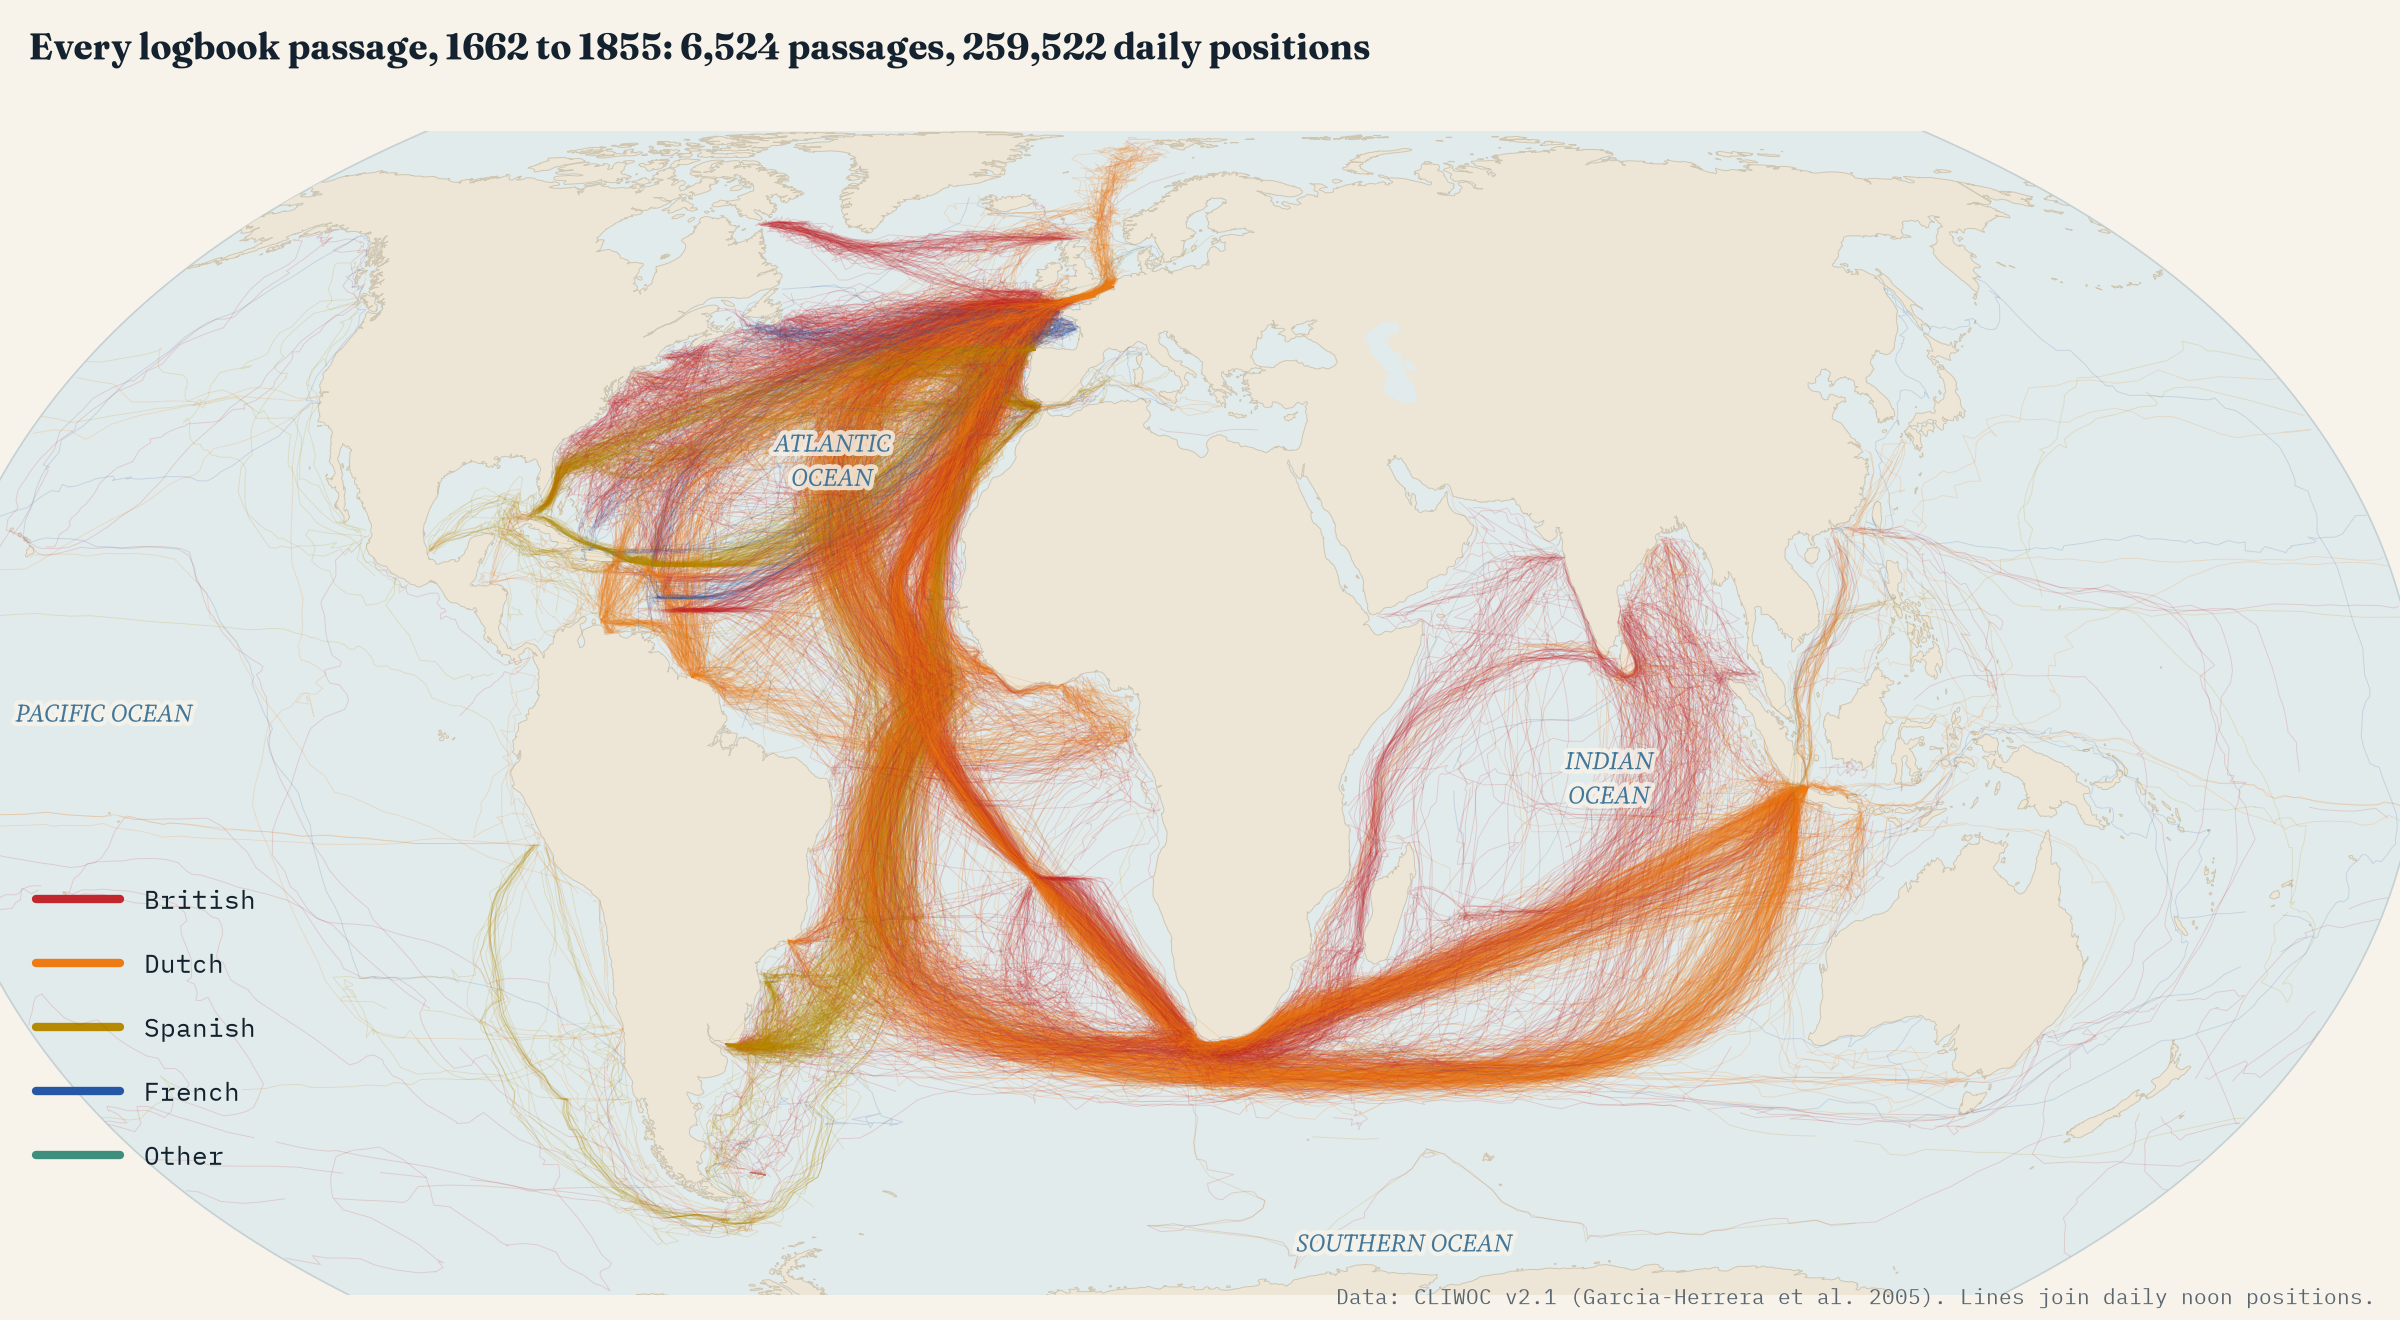
\includegraphics[width=\textwidth]{f_world.png}\caption{Every passage in the record, coloured by nation. Lines join daily positions.}\label{fig:world}\end{figure}

\subsection{Coverage}
Coverage is very uneven in time (Figure~\ref{fig:coverage}, Table~\ref{tab:coverage}). 97\% of Spanish positions date from 1760 to 1799; 67\% of Dutch positions from 1820 or later, many from logbooks held by KNMI; and 73\% of British positions from before 1800, with none after 1829. The busiest decade is the 1770s (42,591 positions) and the thinnest the 1810s (8,192), the years of the Napoleonic Wars. Comparisons across nations or decades therefore compare different kinds of ships in different periods.

\begin{figure}[tbp]\centering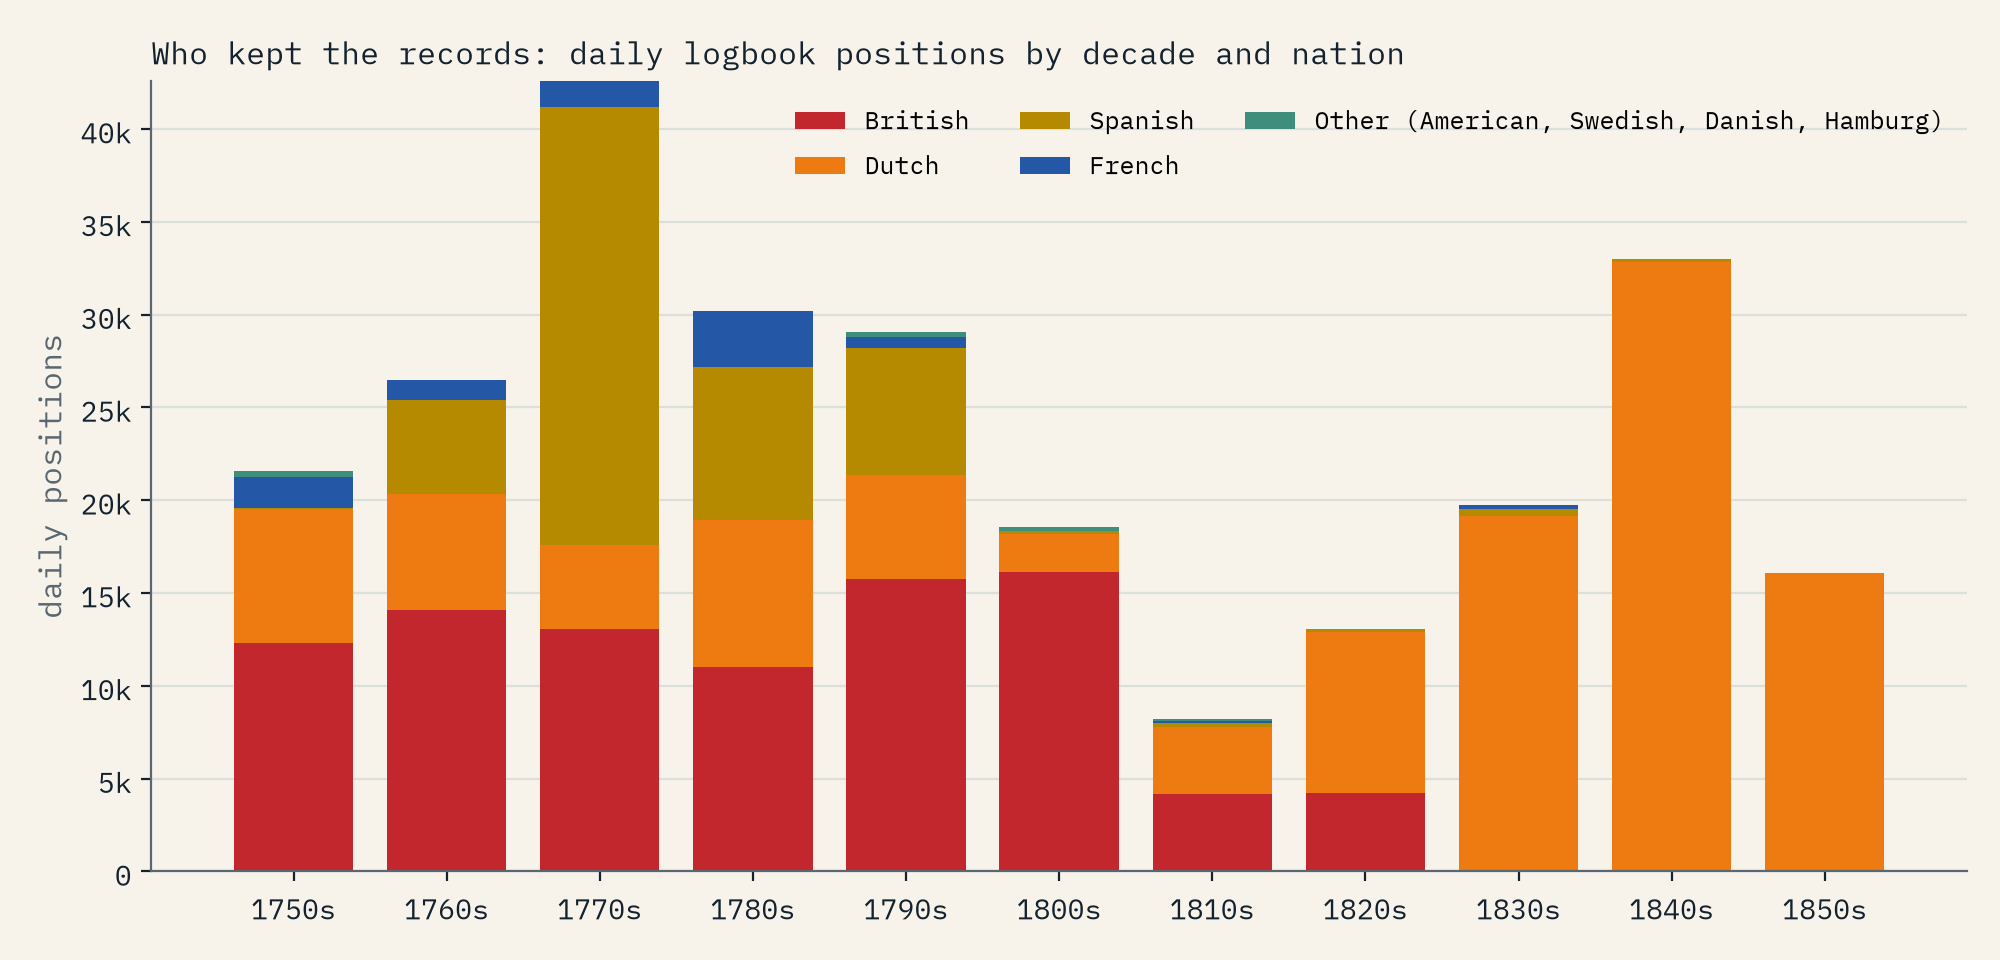
\includegraphics[width=\textwidth]{f_coverage.png}\caption{Daily positions by decade and nation.}\label{fig:coverage}\end{figure}

\begin{table}[tbp]\centering\small\caption{Passages by decade (of their first day) and nation, and daily positions by decade. 14 passages before 1750 are not shown.}\label{tab:coverage}\begin{tabular}{lrrrrrrr}\toprule Decade & British & Dutch & Spanish & French & Other & All & Positions\\\midrule
1750s & 429 & 130 & 2 & 60 & 7 & 628 & 21,586\\
1760s & 457 & 136 & 121 & 39 & 0 & 753 & 26,499\\
1770s & 435 & 95 & 465 & 51 & 0 & 1,046 & 42,591\\
1780s & 300 & 171 & 180 & 90 & 0 & 741 & 30,193\\
1790s & 441 & 116 & 158 & 17 & 7 & 739 & 29,045\\
1800s & 400 & 45 & 7 & 0 & 2 & 454 & 18,553\\
1810s & 87 & 96 & 5 & 7 & 1 & 196 & 8,192\\
1820s & 117 & 261 & 17 & 0 & 0 & 395 & 13,072\\
1830s & 0 & 442 & 5 & 13 & 0 & 460 & 19,736\\
1840s & 0 & 773 & 9 & 0 & 0 & 782 & 33,025\\
1850s & 0 & 316 & 0 & 0 & 0 & 316 & 16,106\\
\bottomrule\end{tabular}\end{table}

\subsection{The volta do mar}
Ships sailing between Europe and the South Atlantic took different roads out and home (Figure~\ref{fig:volta}). At 30° N, 561 outbound crossings had a median longitude of 18° W (interquartile range 17° W to 20° W), and 578 homebound crossings 36° W (34° W to 39° W), 18° further west. At 20° N the medians were 23° W and 34° W. At 38° N, 66\% of homebound crossings lay between 35° W and 20° W, the longitudes of the Azores, against 2\% of outbound ones. Both directions crossed the equator far out in the Atlantic, at a median of 23° W outbound and 21° W homebound, avoiding the calms of the Gulf of Guinea.

\begin{figure}[tbp]\centering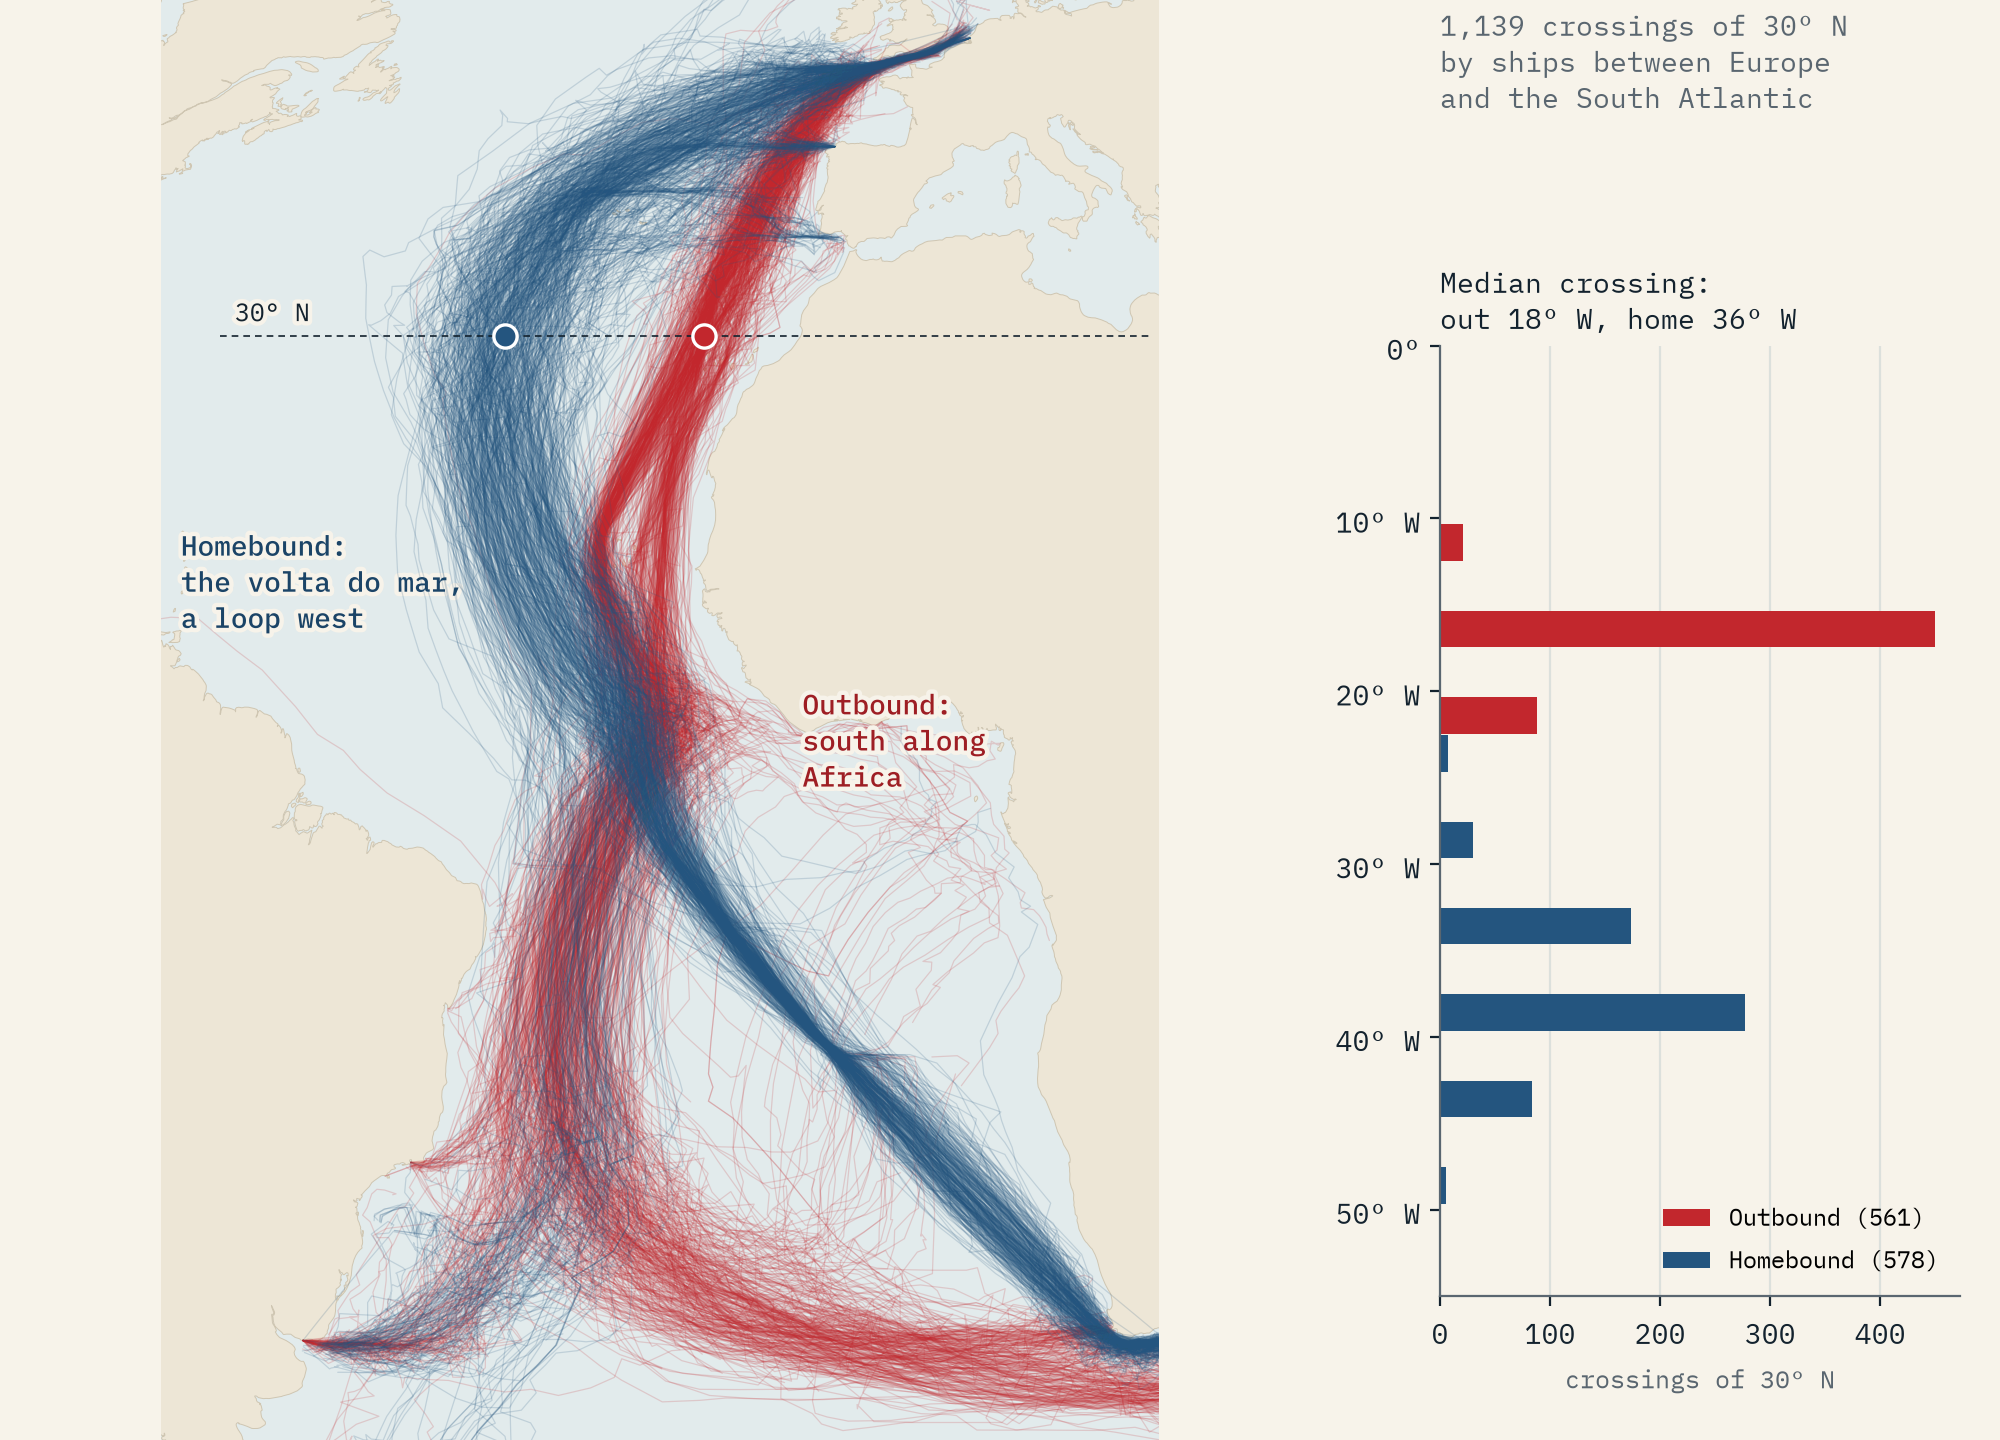
\includegraphics[width=\textwidth]{f_volta.png}\caption{Passages between Europe and the South Atlantic: outbound (red) and homebound (blue), with the median crossing of 30° N in each direction and the distribution of crossings.}\label{fig:volta}\end{figure}

\subsection{The Brouwer route}
From the Cape, Dutch ships ran east in the high southern latitudes (Figure~\ref{fig:brouwer}). Of 323 Dutch eastbound crossings of 75° E, the median latitude was 38° S and 100\% lay south of 30° S; on voyages to Batavia the median Dutch ship reached 40° S between 30° E and 100° E before turning north. British ships also used the westerlies (median 36° S at 75° E, 84\% south of 30° S) but, bound mostly for India, turned north sooner: at 90° E the British median was 15° S against 34° S for the Dutch.

\begin{figure}[tbp]\centering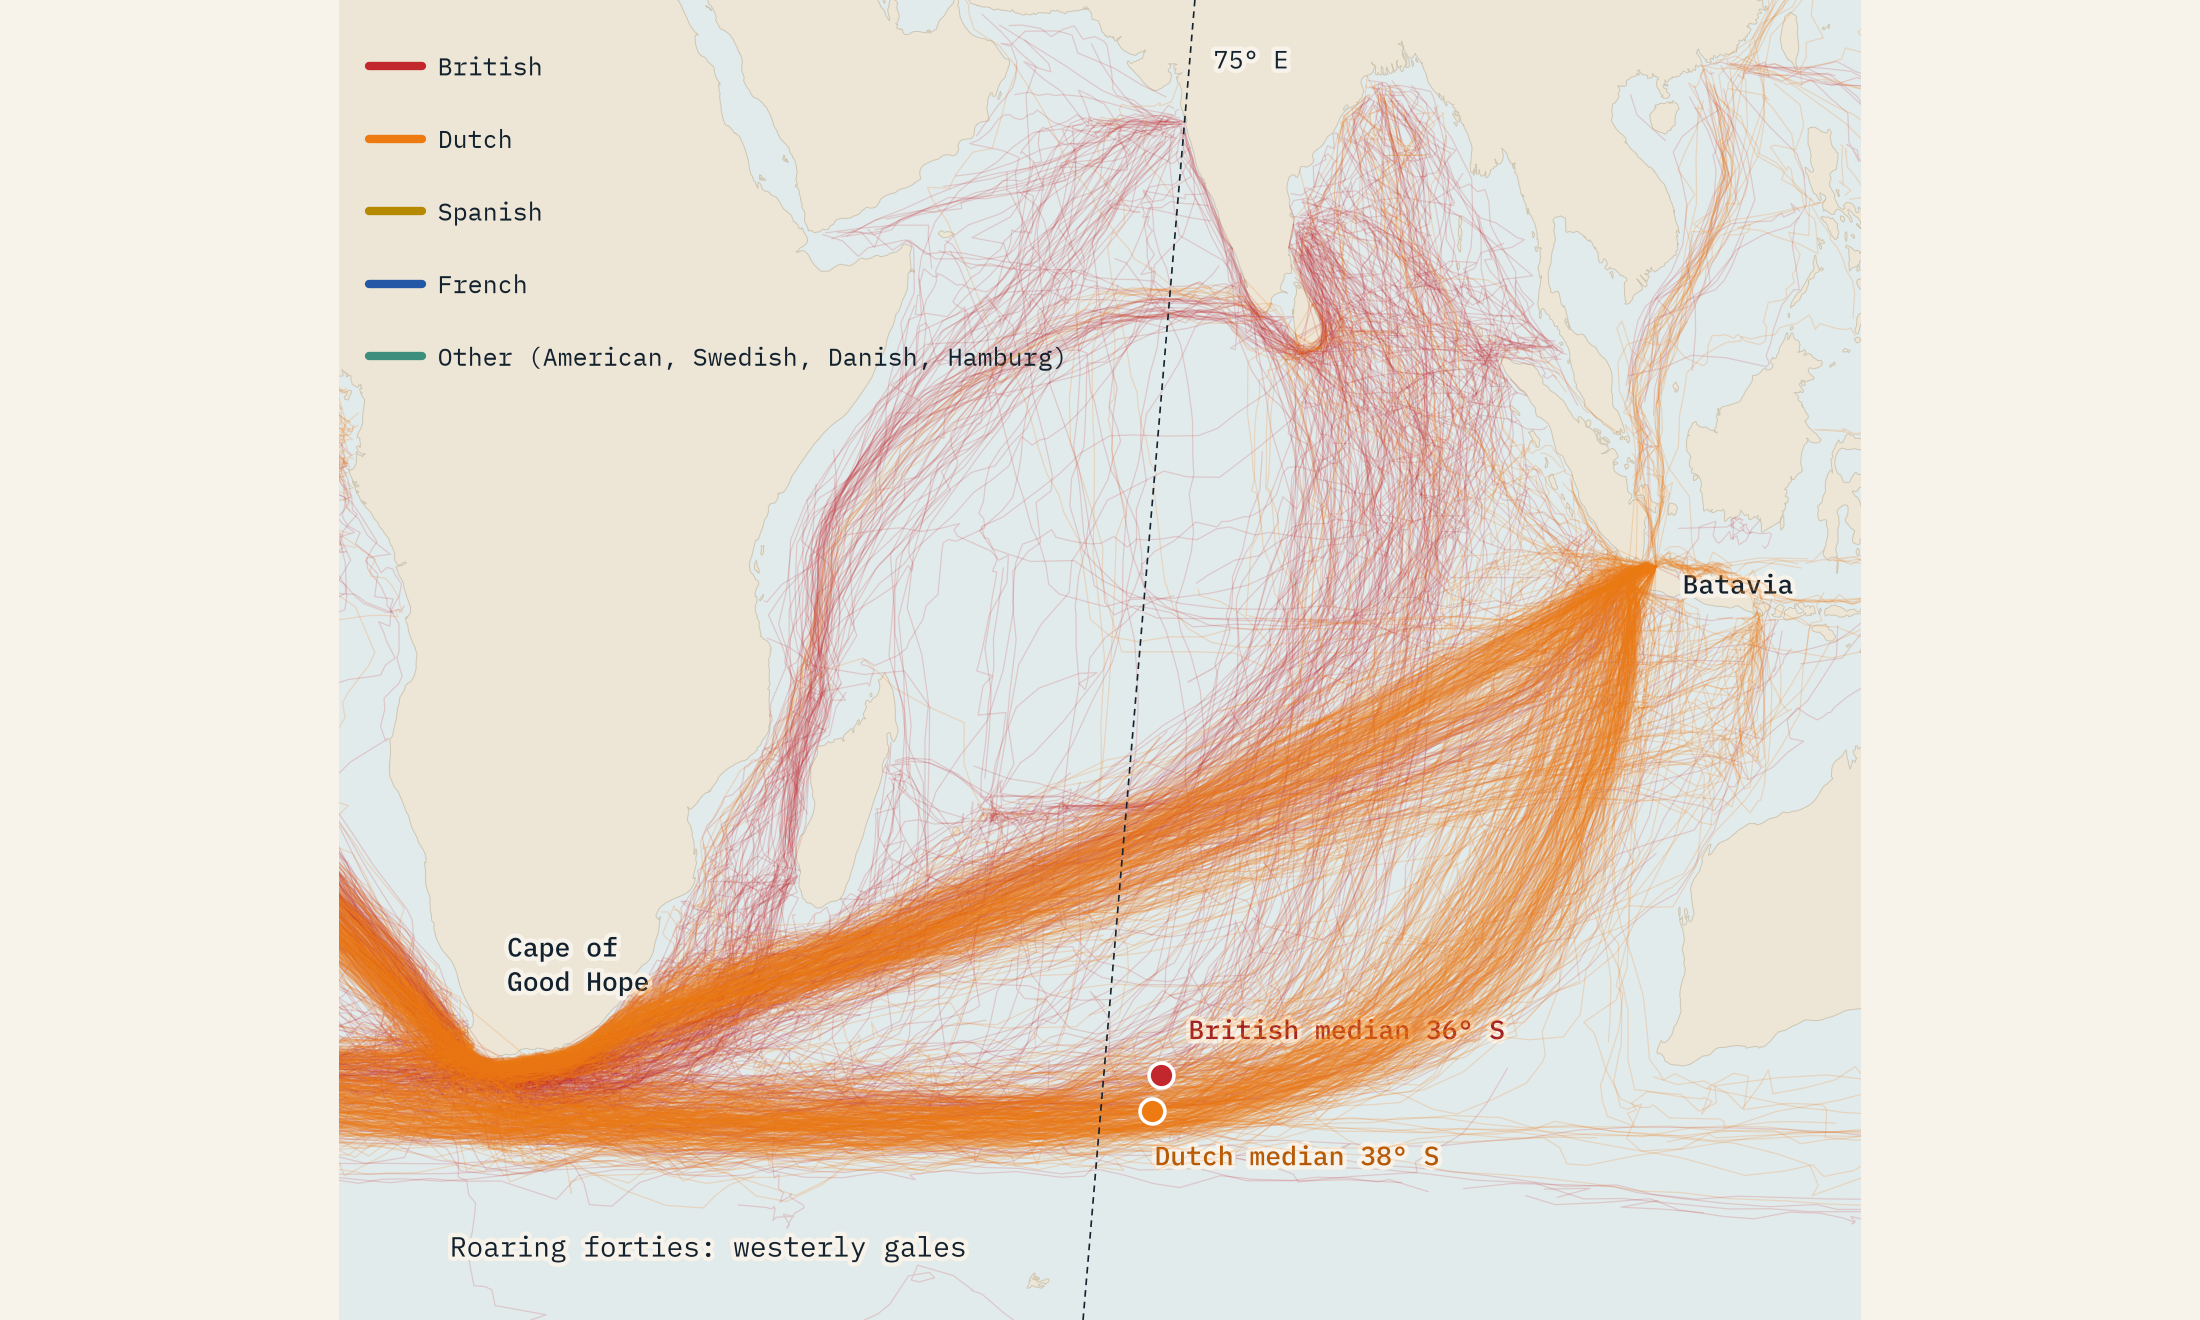
\includegraphics[width=\textwidth]{f_brouwer.png}\caption{British and Dutch passages in the Indian Ocean, with the median latitude of eastbound crossings of 75° E.}\label{fig:brouwer}\end{figure}

\subsection{Voyage times}
Table~\ref{tab:dur} and Figure~\ref{fig:dur} give voyage times. The most frequent long voyage in the record, home waters to Batavia, took a median of 102 days (219 voyages, quartiles 94 and 119); 44 called at the Cape. The 15 voyages before 1820 had a median of 176 days and those from 1820 on 101, 43\% shorter. Some of the difference is the long stay at the Cape made by Company ships, but the Cape to Batavia leg alone fell from 71 to 45 days. The early figures rest on few voyages. On the Spanish mail routes the downwind run from La Coruña or Cádiz to Puerto Rico took 38 days and the return from Havana 81.

\begin{table}[tbp]\centering\small\caption{Voyage times in days, from the last position at the start to the first at the destination.}\label{tab:dur}\begin{tabular}{>{\raggedright\arraybackslash}p{6.4cm}rrrrr}\toprule Route & Voyages & Median & Middle half & Fastest & Years\\\midrule
Home waters to Batavia & 219 & 102 & 94 to 119 & 80 & 1662 to 1854\\
Batavia to home waters & 131 & 110 & 100 to 120 & 82 & 1819 to 1854\\
Home waters to the Cape & 79 & 85 & 68 to 98 & 50 & 1662 to 1853\\
Cape to Batavia & 54 & 52 & 43 to 62 & 33 & 1663 to 1853\\
Home waters to Suriname & 40 & 35 & 30 to 40 & 21 & 1759 to 1852\\
Home waters to India (Bombay, Madras, Bengal) & 18 & 133 & 118 to 172 & 103 & 1754 to 1825\\
India to home waters & 7 & 171 & 150 to 174 & 145 & 1764 to 1813\\
Home waters to the Caribbean & 27 & 38 & 31 to 41 & 21 & 1752 to 1822\\
Home waters to Halifax and New York & 8 & 44 & 36 to 53 & 32 & 1753 to 1790\\
Cádiz or La Coruña to Puerto Rico & 12 & 38 & 35 to 42 & 29 & 1766 to 1796\\
Cádiz or La Coruña to Havana & 4 & 54 & 48 to 67 & 46 & 1766 to 1776\\
Havana to Cádiz or La Coruña & 15 & 81 & 45 to 92 & 27 & 1765 to 1794\\
Cádiz or La Coruña to the River Plate & 14 & 70 & 65 to 74 & 61 & 1769 to 1793\\
River Plate to Cádiz or La Coruña & 6 & 91 & 80 to 117 & 76 & 1773 to 1798\\
\bottomrule\end{tabular}\end{table}

\begin{figure}[tbp]\centering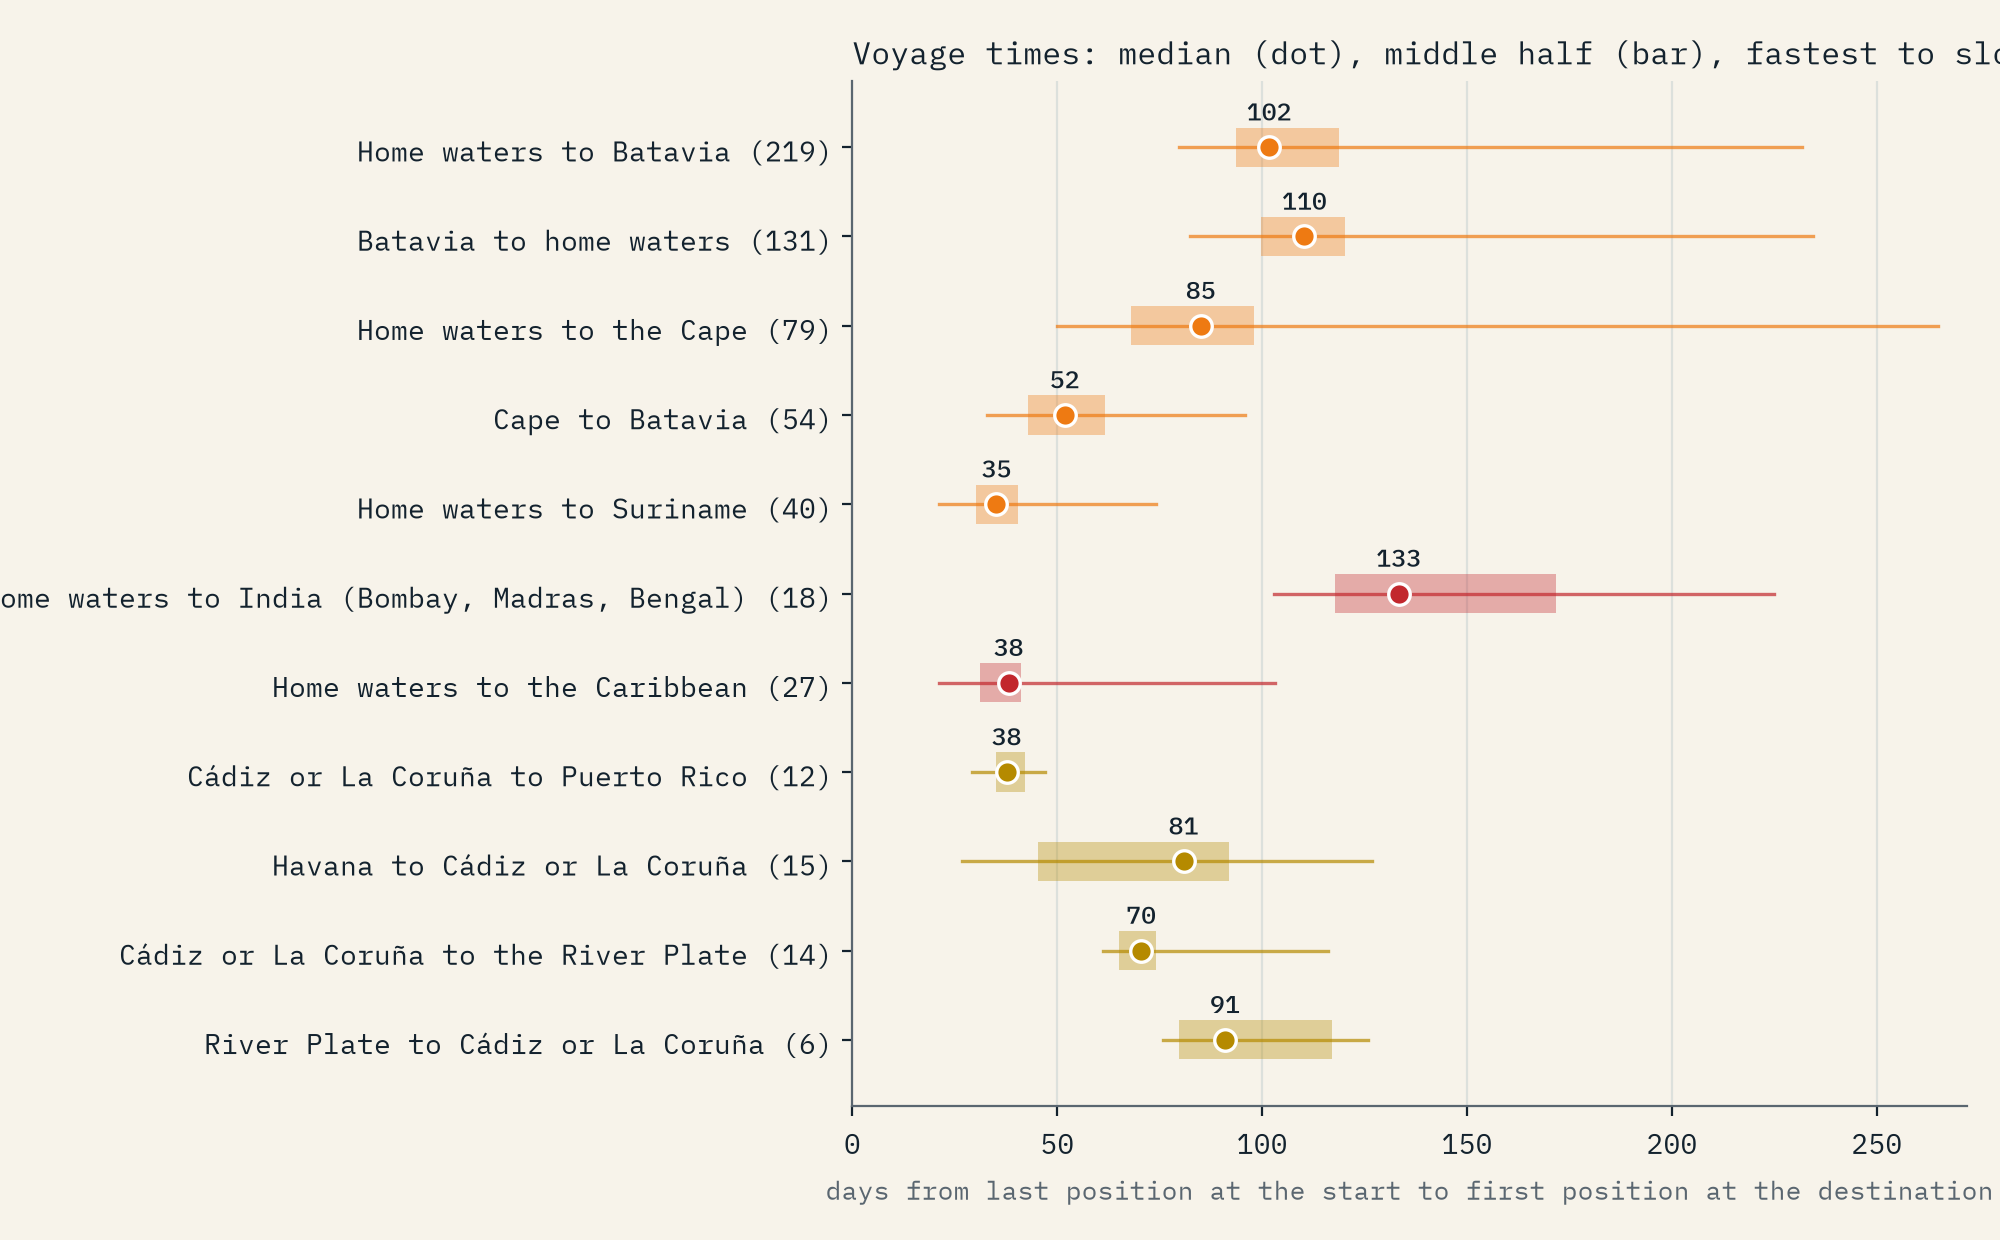
\includegraphics[width=\textwidth]{f_durations.png}\caption{Voyage times on the great routes: median, interquartile range and range.}\label{fig:dur}\end{figure}

\subsection{Busiest routes}
Legs between named places show each nation's network. The busiest route is between European home waters and Batavia (252 legs, 236 Dutch), then home waters and the Cape (242) and the Cape and Batavia (103). Dutch logbooks also trace the Atlantic triangle of the Middelburgsche Commercie Compagnie, which carried enslaved Africans from the Gold Coast to Suriname and the Caribbean: home waters to Suriname (60 legs) and the Gold Coast to home waters (37). Spanish logbooks run from La Coruña and Cádiz to the River Plate, Puerto Rico and Havana; British ones, mostly naval, to the Cape, Barbados and Ceylon. The full table is in the data release.

\subsection{Winds}
The logbook winds reproduce the global wind belts (Figure~\ref{fig:winds}). In the Atlantic, 73\% of winds between 10° and 25° N and 60° W and 15° W came from between north and east, and 68\% between 5° and 25° S from between east and south. In the southern Indian Ocean between 36° and 48° S, 70\% came from a westerly point, with a mean force of 9.3 m/s against 4.6 m/s between the equator and 5° N in the Atlantic, where 7.9\% of entries were calm or variable, 2.9 times the rate in the trade-wind belts. The monsoon reverses as expected (Figure~\ref{fig:monsoon}): in the northern Indian Ocean 65\% of December to February winds came from the north-east quadrant and 81\% of June to August winds from the south-west.

Against the modern reanalysis, the mean logbook direction lies within 45° of the benchmark in 97\% of the 318 squares where the benchmark wind is steady (mean vector at least 3 m/s), and within 30° in 93\%, with a median difference of 9°; over all 537 squares the share within 45° is 88\%. Individual daily entries are noisier: 65\% lie within 45° of the monthly benchmark. Across 39 latitude bands the west-to-east components of the logbook and benchmark winds correlate at 0.93 and share a sign in 92\%. The logbook westerlies look weaker than the benchmark's because daily winds vary much more in direction than monthly means; directions agree better than steadiness.

\begin{figure}[tbp]\centering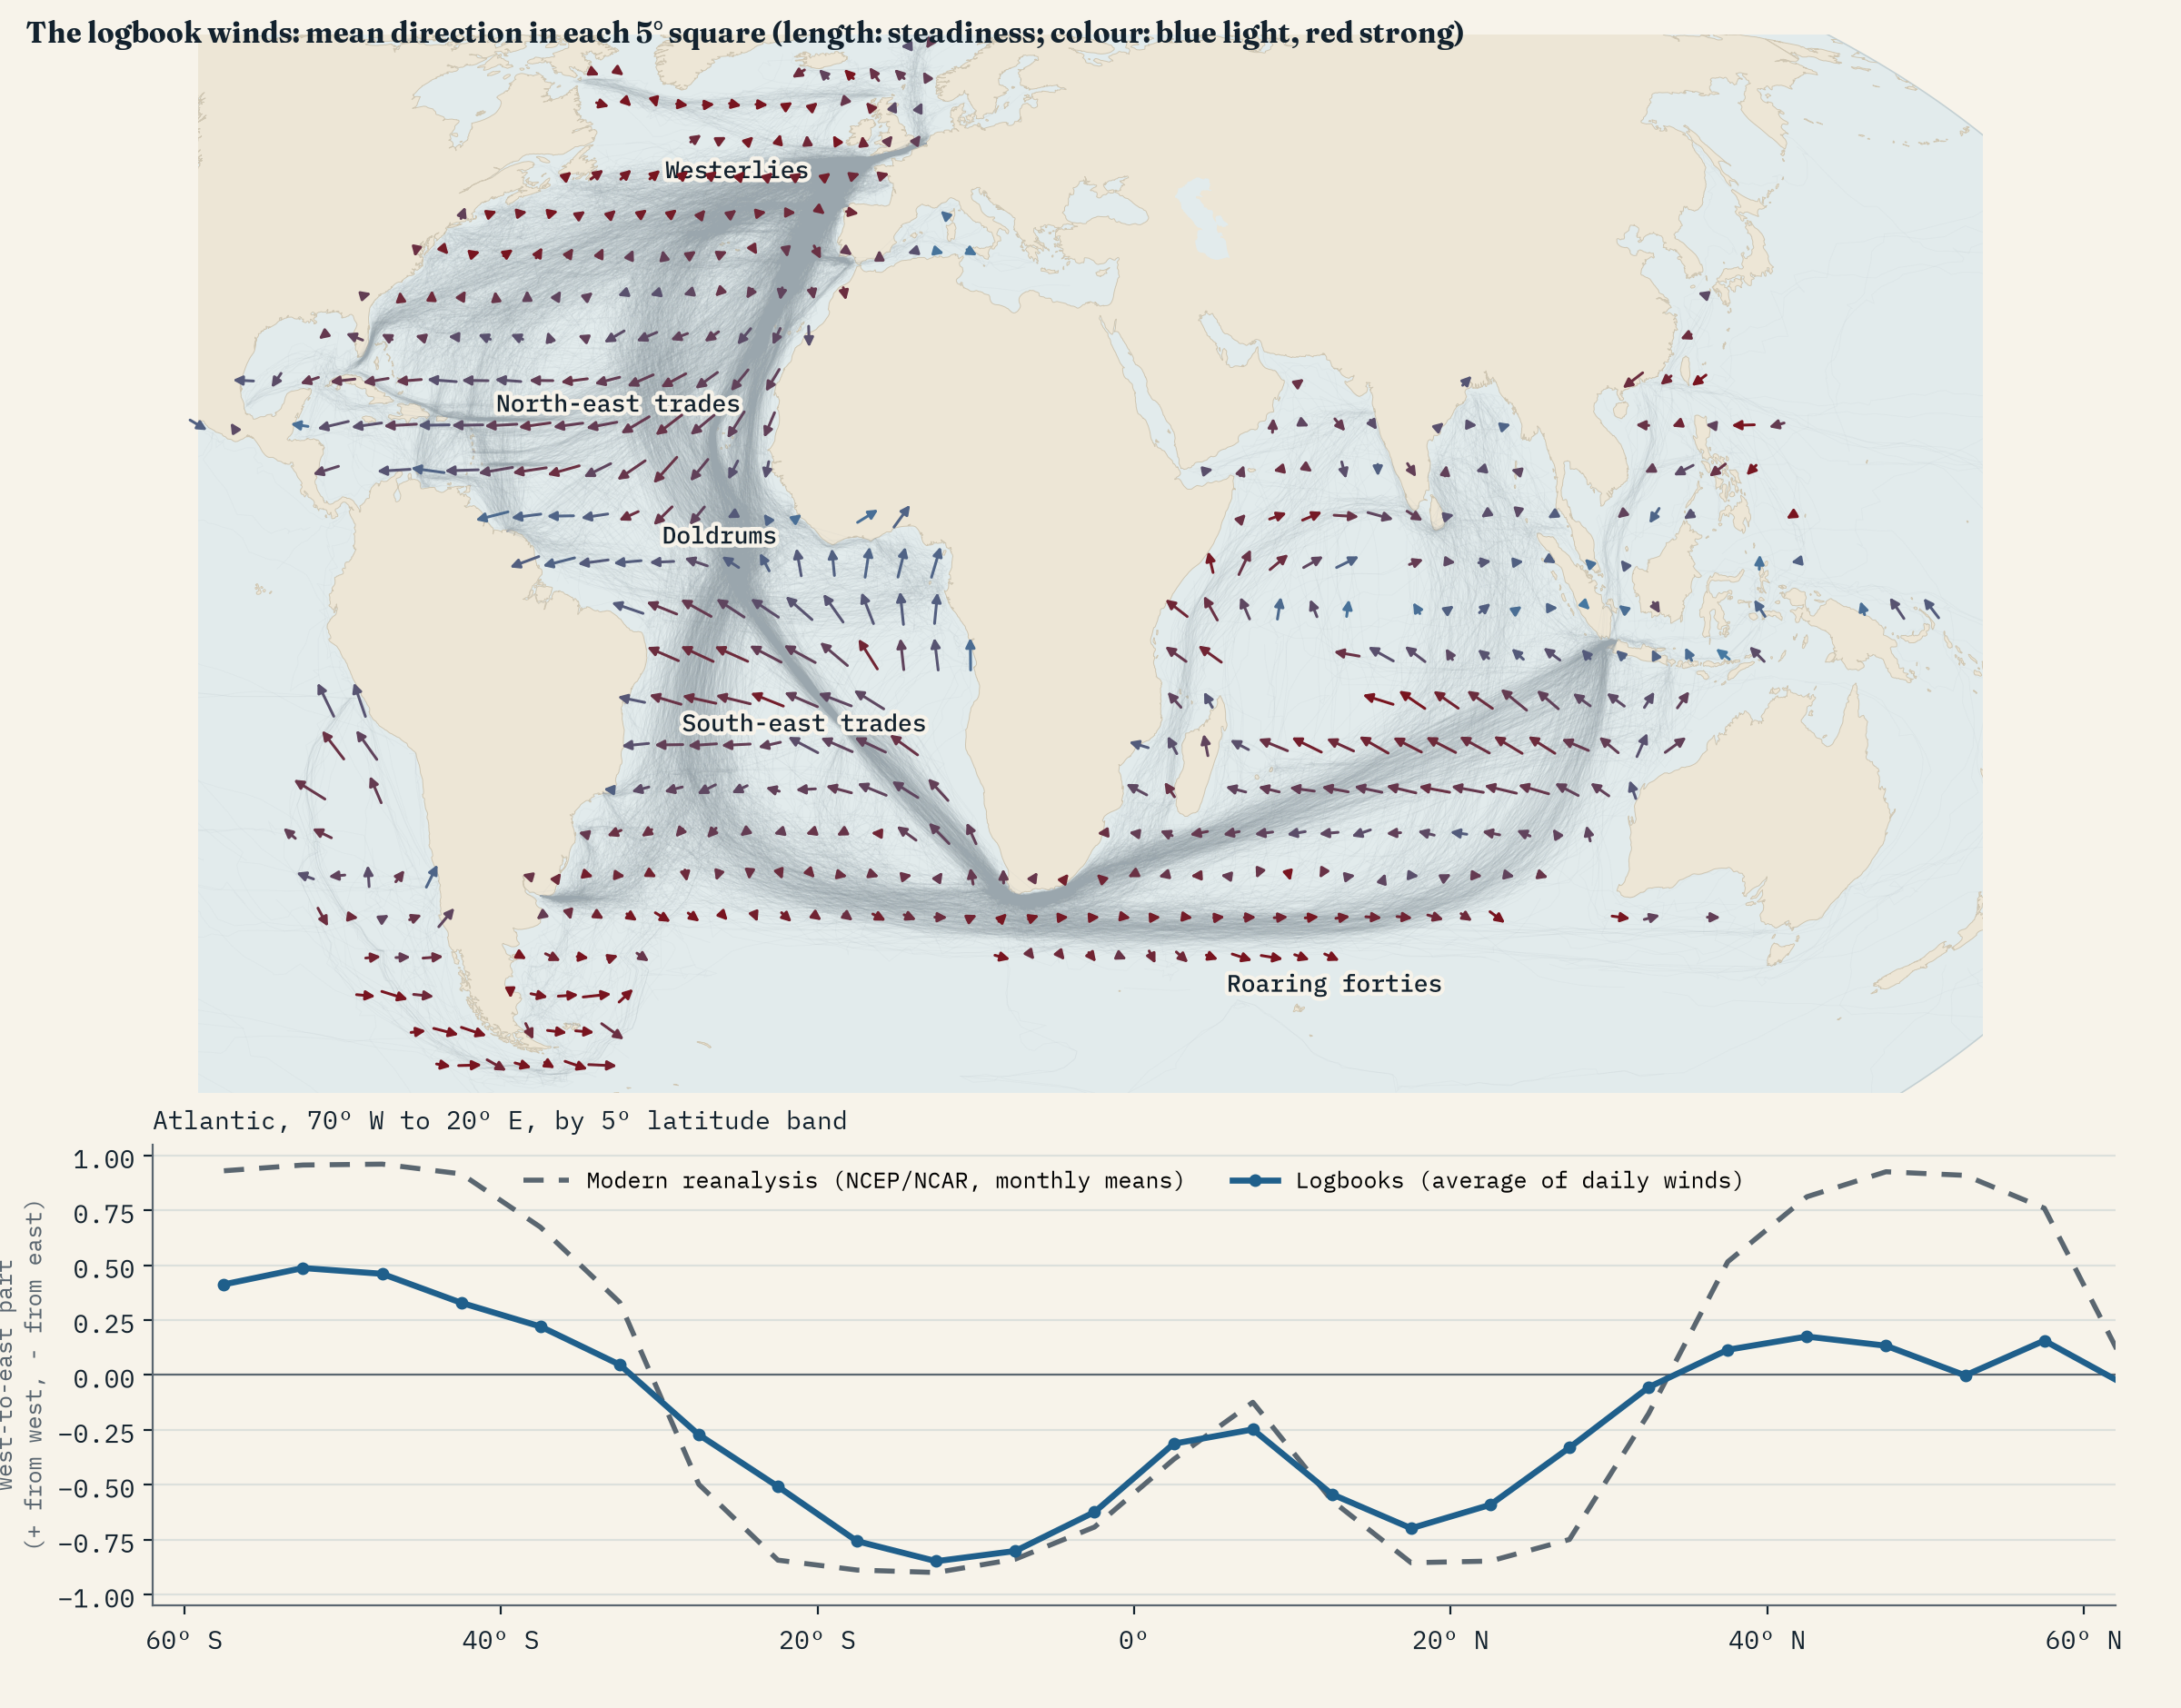
\includegraphics[width=\textwidth]{f_winds.png}\caption{Top: mean logbook wind direction in each 5° square with at least 25 entries (length: steadiness; colour: force). Bottom: west-to-east component by latitude in the Atlantic, logbooks and the modern reanalysis.}\label{fig:winds}\end{figure}

\begin{figure}[tbp]\centering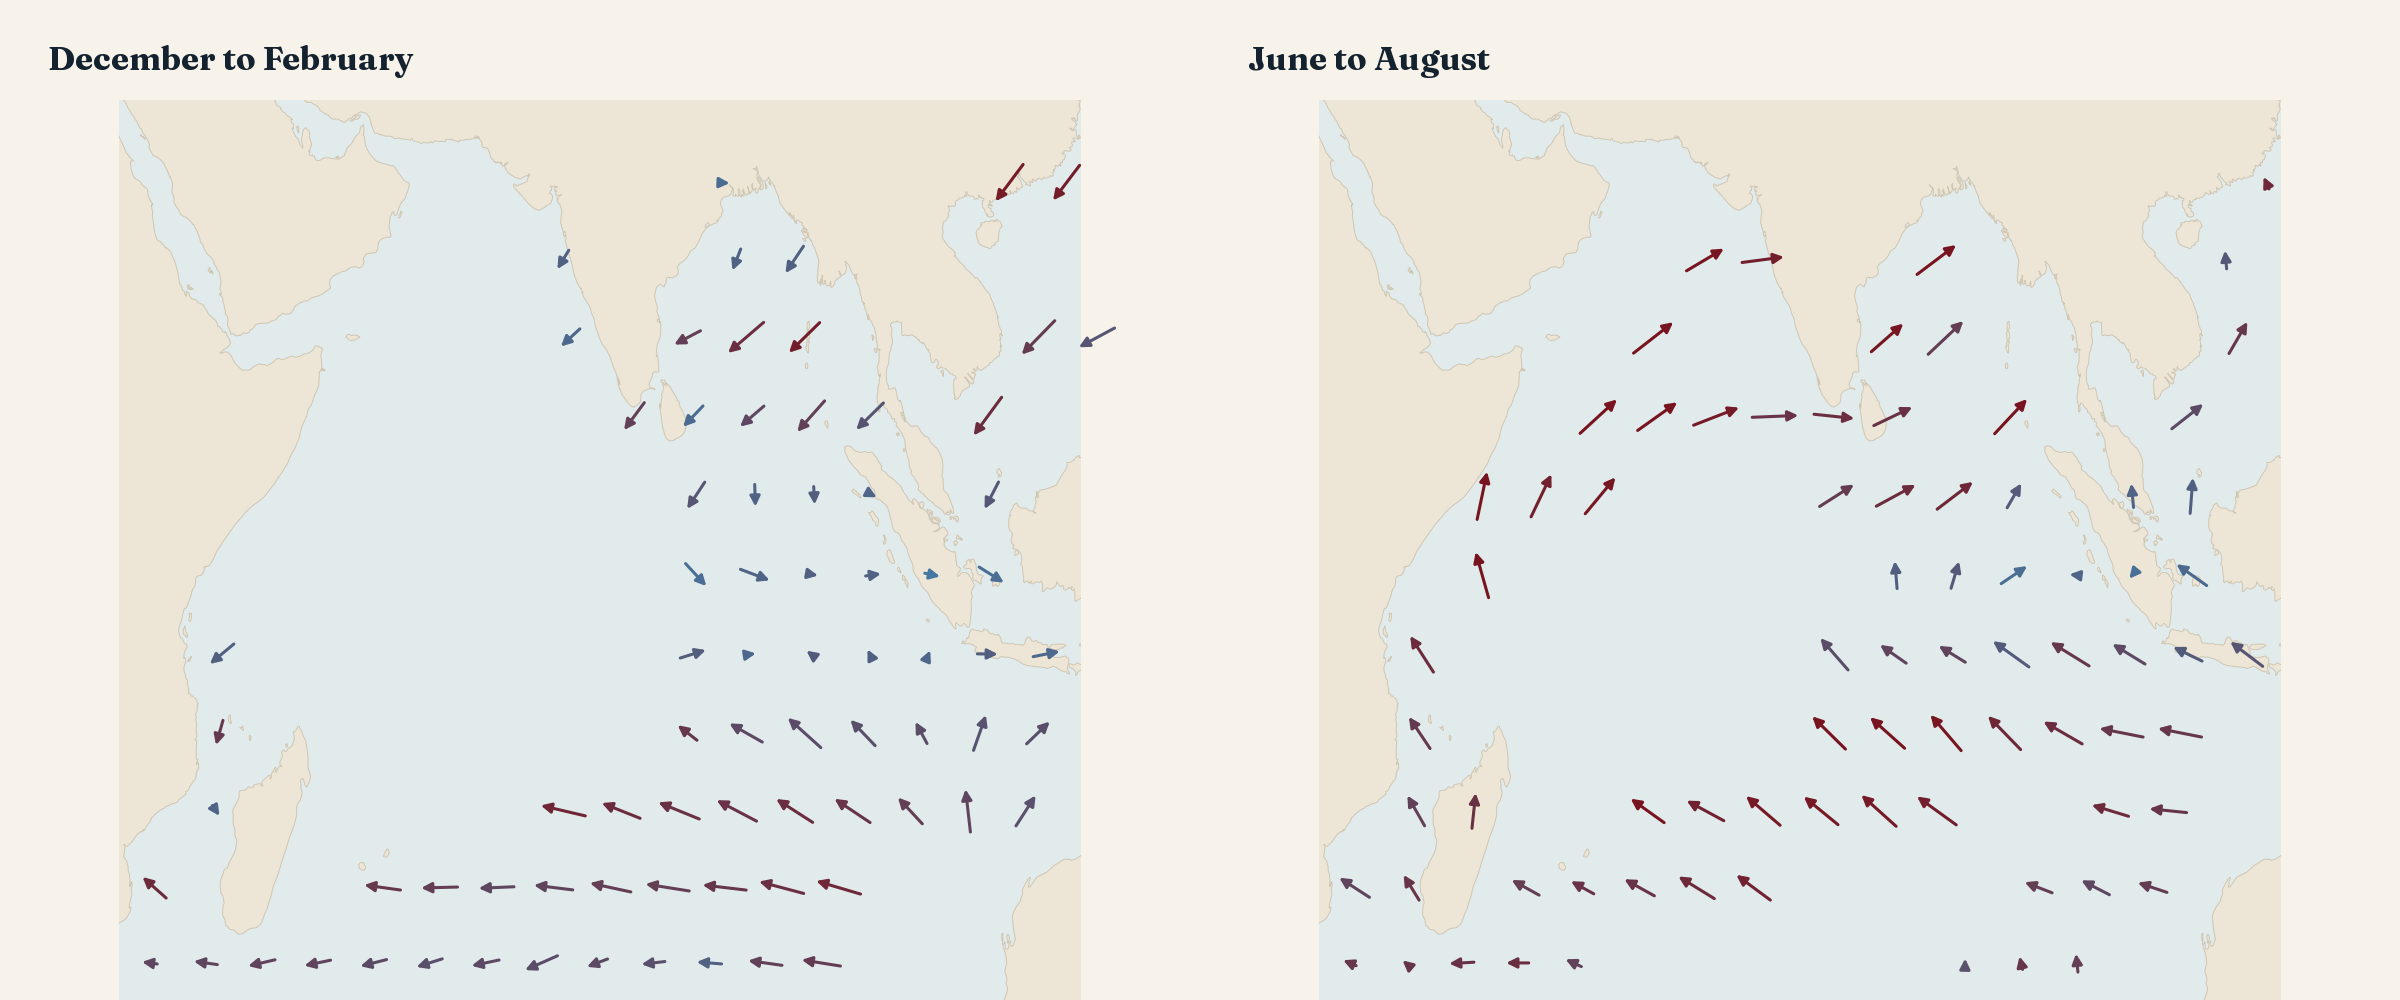
\includegraphics[width=\textwidth]{f_monsoon.png}\caption{Logbook winds in the Indian Ocean in December to February and June to August.}\label{fig:monsoon}\end{figure}

\subsection{Then and now}
The sailing routes differ from today's shipping lanes (Figure~\ref{fig:now}). Over 2° squares the rank correlation between logbook passages and the AIS traffic index is 0.22. The southern Indian Ocean between 35° and 50° S holds 5.9\% of the logbook record and about 0.00\% of today's traffic index; the mid South Atlantic 13.9\% against 0.5\%. The Red Sea and Gulf of Aden carry 1.3\% of today's traffic and 0.01\% of the logbook record, and 31\% of the busiest tenth of today's squares were crossed by no logbook ship. Because the logbooks are a sample and AIS reception varies, these are rough contrasts.

\begin{figure}[tbp]\centering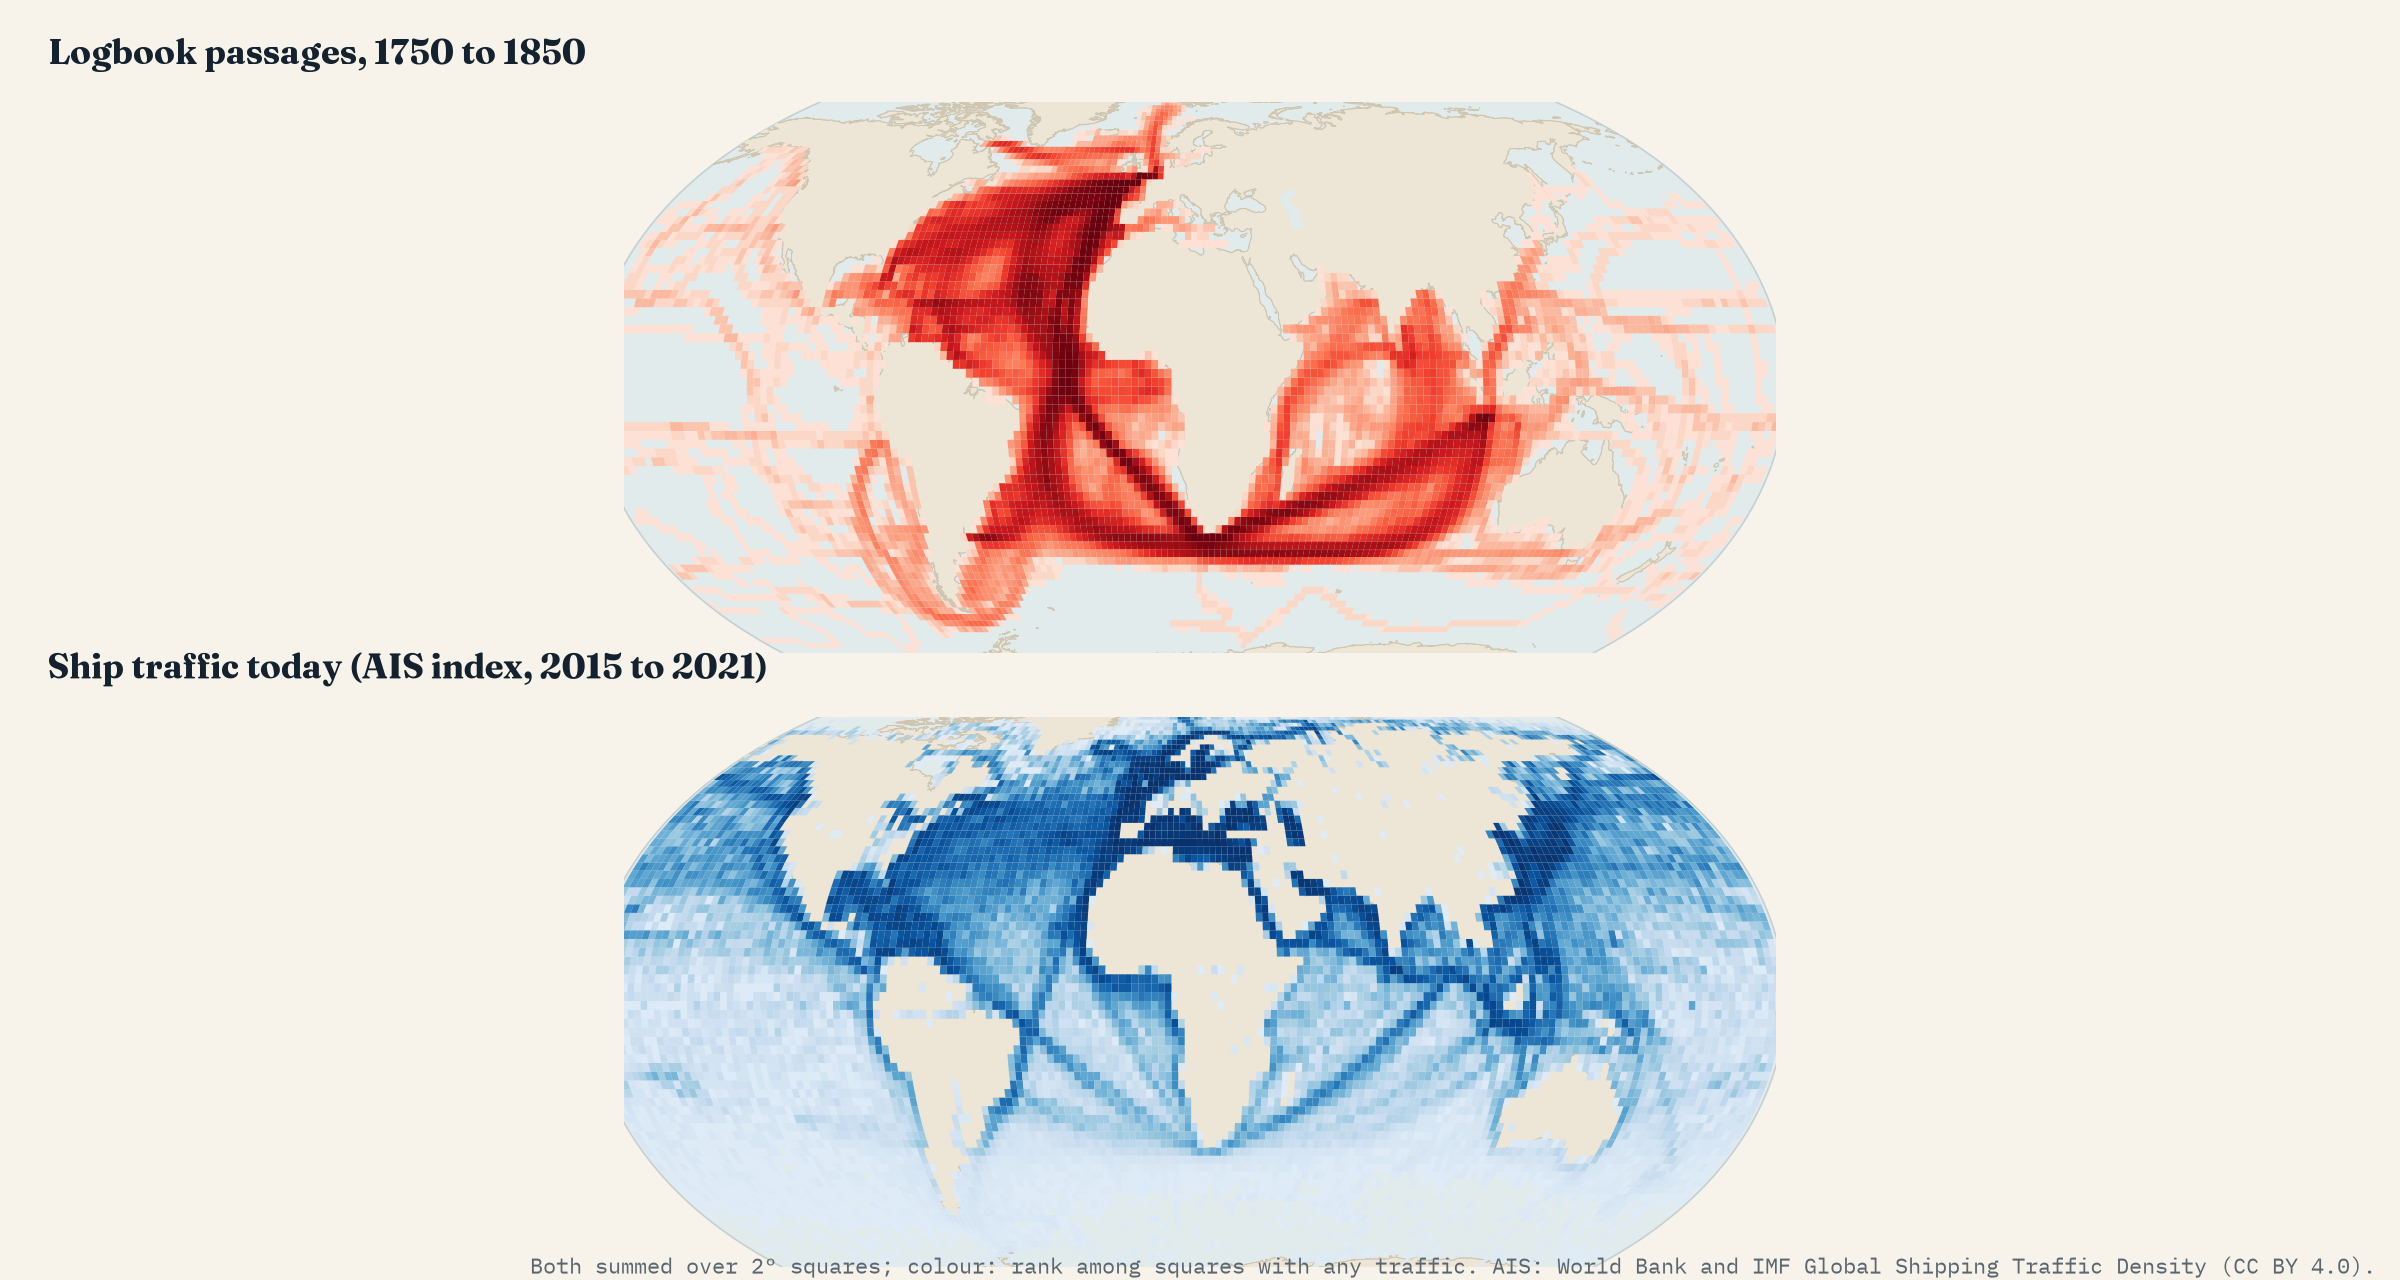
\includegraphics[width=\textwidth]{f_thennow.png}\caption{Logbook passages (top) and ship traffic today (bottom), by 2° square; colour shows each square's rank among squares with any traffic.}\label{fig:now}\end{figure}

\section{Limitations}
The record is a sample of logbooks that survived, were archived in four countries and were chosen for digitisation, so it is dominated by navies and by particular periods for each nation; Portuguese, American, Danish and Swedish shipping and most merchant shipping are missing, and the Pacific is nearly empty. Comparisons across time mix changes in shipping with changes in which logbooks survive. Positions are dead-reckoning estimates with errors of tens of kilometres or more, especially in longitude before chronometers, and daily positions joined by straight lines are not the ship's true track. Port matching uses generous circles and boxes, so a ship passing close to a port can count as calling there, and voyage times begin when the log last places the ship in port or home waters. Wind directions and forces were translated from historical terms and compass points, whose accuracy varies between logbooks \citep{wheeler2005}; the benchmark is a modern reanalysis, so differences also reflect real change and model error. The AIS comparison uses a sampled overview raster and is only indicative.

\section*{Data availability}
Derived data (logbook records, passages with daily positions, voyages and durations, routes, crossings, wind grids and belts, coverage by decade, 2° squares and the full results) and all code are at \url{https://github.com/Tristan-Hotham/ships-before-steam} and archived with this paper. The text, figures and derived data are shared under CC BY 4.0 and the code under MIT. The logbook positions derive from CLIWOC v2.1, openly published research data for which I found no formal licence; anyone reusing them should credit \citet{garciaherrera2005} and check the original terms.

\section*{AI statement}
I wrote the text, with drafting and editing assistance from Claude (Anthropic), which also helped prepare the analysis code. I reviewed and checked all text and results.

\begin{thebibliography}{99}
\bibitem[Bruijn et al.(1987)]{bruijn1987} Bruijn, J.R., Gaastra, F.S. and Schöffer, I. (1987) \emph{Dutch-Asiatic Shipping in the 17th and 18th Centuries}. The Hague: Martinus Nijhoff.
\bibitem[Cerdeiro et al.(2020)]{cerdeiro2020} Cerdeiro, D.A., Komaromi, A., Liu, Y. and Saeed, M. (2020) World seaborne trade in real time: a proof of concept for building AIS-based nowcasts from scratch. IMF Working Paper 20/57. Data: World Bank, Global Shipping Traffic Density, CC BY 4.0.
\bibitem[Correoso(n.d.)]{correoso} Correoso, F. (n.d.) cliwoc\_vis: CLIWOC visualisation and GeoJSON of CLIWOC voyages. \url{https://github.com/kikocorreoso/cliwoc_vis}
\bibitem[Garc\'ia-Herrera et al.(2005)]{garciaherrera2005} García-Herrera, R., Können, G.P., Wheeler, D.A., Prieto, M.R., Jones, P.D. and Koek, F.B. (2005) CLIWOC: a climatological database for the world's oceans 1750 to 1854. \emph{Climatic Change} 73, 1 to 12.
\bibitem[Kalnay et al.(1996)]{kalnay1996} Kalnay, E. et al. (1996) The NCEP/NCAR 40-year reanalysis project. \emph{Bulletin of the American Meteorological Society} 77, 437 to 471.
\bibitem[Küttel et al.(2010)]{kuttel2010} Küttel, M., Xoplaki, E., Gallego, D., Luterbacher, J., García-Herrera, R., Allan, R., Barriendos, M., Jones, P.D., Wheeler, D. and Wanner, H. (2010) The importance of ship log data: reconstructing North Atlantic, European and Mediterranean sea level pressure fields back to 1750. \emph{Climate Dynamics} 34, 1115 to 1128.
\bibitem[Wheeler(2005)]{wheeler2005} Wheeler, D. (2005) An examination of the accuracy and consistency of ships' logbook weather observations and records. \emph{Climatic Change} 73, 97 to 116.
\end{thebibliography}
\end{document}
